\documentclass[]{article}
\usepackage{lmodern}
\usepackage{amssymb,amsmath}
\usepackage{ifxetex,ifluatex}
\usepackage{fixltx2e} % provides \textsubscript
\ifnum 0\ifxetex 1\fi\ifluatex 1\fi=0 % if pdftex
  \usepackage[T1]{fontenc}
  \usepackage[utf8]{inputenc}
\else % if luatex or xelatex
  \ifxetex
    \usepackage{mathspec}
  \else
    \usepackage{fontspec}
  \fi
  \defaultfontfeatures{Ligatures=TeX,Scale=MatchLowercase}
\fi
% use upquote if available, for straight quotes in verbatim environments
\IfFileExists{upquote.sty}{\usepackage{upquote}}{}
% use microtype if available
\IfFileExists{microtype.sty}{%
\usepackage{microtype}
\UseMicrotypeSet[protrusion]{basicmath} % disable protrusion for tt fonts
}{}
\usepackage[margin=1in]{geometry}
\usepackage{hyperref}
\hypersetup{unicode=true,
            pdftitle={A Brief Introduction to Bandwidth Selection Methods for Univariate Kernel Density Estimation},
            pdfauthor={Brad Stieber},
            pdfborder={0 0 0},
            breaklinks=true}
\urlstyle{same}  % don't use monospace font for urls
\usepackage{color}
\usepackage{fancyvrb}
\newcommand{\VerbBar}{|}
\newcommand{\VERB}{\Verb[commandchars=\\\{\}]}
\DefineVerbatimEnvironment{Highlighting}{Verbatim}{commandchars=\\\{\}}
% Add ',fontsize=\small' for more characters per line
\usepackage{framed}
\definecolor{shadecolor}{RGB}{248,248,248}
\newenvironment{Shaded}{\begin{snugshade}}{\end{snugshade}}
\newcommand{\KeywordTok}[1]{\textcolor[rgb]{0.13,0.29,0.53}{\textbf{{#1}}}}
\newcommand{\DataTypeTok}[1]{\textcolor[rgb]{0.13,0.29,0.53}{{#1}}}
\newcommand{\DecValTok}[1]{\textcolor[rgb]{0.00,0.00,0.81}{{#1}}}
\newcommand{\BaseNTok}[1]{\textcolor[rgb]{0.00,0.00,0.81}{{#1}}}
\newcommand{\FloatTok}[1]{\textcolor[rgb]{0.00,0.00,0.81}{{#1}}}
\newcommand{\ConstantTok}[1]{\textcolor[rgb]{0.00,0.00,0.00}{{#1}}}
\newcommand{\CharTok}[1]{\textcolor[rgb]{0.31,0.60,0.02}{{#1}}}
\newcommand{\SpecialCharTok}[1]{\textcolor[rgb]{0.00,0.00,0.00}{{#1}}}
\newcommand{\StringTok}[1]{\textcolor[rgb]{0.31,0.60,0.02}{{#1}}}
\newcommand{\VerbatimStringTok}[1]{\textcolor[rgb]{0.31,0.60,0.02}{{#1}}}
\newcommand{\SpecialStringTok}[1]{\textcolor[rgb]{0.31,0.60,0.02}{{#1}}}
\newcommand{\ImportTok}[1]{{#1}}
\newcommand{\CommentTok}[1]{\textcolor[rgb]{0.56,0.35,0.01}{\textit{{#1}}}}
\newcommand{\DocumentationTok}[1]{\textcolor[rgb]{0.56,0.35,0.01}{\textbf{\textit{{#1}}}}}
\newcommand{\AnnotationTok}[1]{\textcolor[rgb]{0.56,0.35,0.01}{\textbf{\textit{{#1}}}}}
\newcommand{\CommentVarTok}[1]{\textcolor[rgb]{0.56,0.35,0.01}{\textbf{\textit{{#1}}}}}
\newcommand{\OtherTok}[1]{\textcolor[rgb]{0.56,0.35,0.01}{{#1}}}
\newcommand{\FunctionTok}[1]{\textcolor[rgb]{0.00,0.00,0.00}{{#1}}}
\newcommand{\VariableTok}[1]{\textcolor[rgb]{0.00,0.00,0.00}{{#1}}}
\newcommand{\ControlFlowTok}[1]{\textcolor[rgb]{0.13,0.29,0.53}{\textbf{{#1}}}}
\newcommand{\OperatorTok}[1]{\textcolor[rgb]{0.81,0.36,0.00}{\textbf{{#1}}}}
\newcommand{\BuiltInTok}[1]{{#1}}
\newcommand{\ExtensionTok}[1]{{#1}}
\newcommand{\PreprocessorTok}[1]{\textcolor[rgb]{0.56,0.35,0.01}{\textit{{#1}}}}
\newcommand{\AttributeTok}[1]{\textcolor[rgb]{0.77,0.63,0.00}{{#1}}}
\newcommand{\RegionMarkerTok}[1]{{#1}}
\newcommand{\InformationTok}[1]{\textcolor[rgb]{0.56,0.35,0.01}{\textbf{\textit{{#1}}}}}
\newcommand{\WarningTok}[1]{\textcolor[rgb]{0.56,0.35,0.01}{\textbf{\textit{{#1}}}}}
\newcommand{\AlertTok}[1]{\textcolor[rgb]{0.94,0.16,0.16}{{#1}}}
\newcommand{\ErrorTok}[1]{\textcolor[rgb]{0.64,0.00,0.00}{\textbf{{#1}}}}
\newcommand{\NormalTok}[1]{{#1}}
\usepackage{graphicx,grffile}
\makeatletter
\def\maxwidth{\ifdim\Gin@nat@width>\linewidth\linewidth\else\Gin@nat@width\fi}
\def\maxheight{\ifdim\Gin@nat@height>\textheight\textheight\else\Gin@nat@height\fi}
\makeatother
% Scale images if necessary, so that they will not overflow the page
% margins by default, and it is still possible to overwrite the defaults
% using explicit options in \includegraphics[width, height, ...]{}
\setkeys{Gin}{width=\maxwidth,height=\maxheight,keepaspectratio}
\IfFileExists{parskip.sty}{%
\usepackage{parskip}
}{% else
\setlength{\parindent}{0pt}
\setlength{\parskip}{6pt plus 2pt minus 1pt}
}
\setlength{\emergencystretch}{3em}  % prevent overfull lines
\providecommand{\tightlist}{%
  \setlength{\itemsep}{0pt}\setlength{\parskip}{0pt}}
\setcounter{secnumdepth}{0}
% Redefines (sub)paragraphs to behave more like sections
\ifx\paragraph\undefined\else
\let\oldparagraph\paragraph
\renewcommand{\paragraph}[1]{\oldparagraph{#1}\mbox{}}
\fi
\ifx\subparagraph\undefined\else
\let\oldsubparagraph\subparagraph
\renewcommand{\subparagraph}[1]{\oldsubparagraph{#1}\mbox{}}
\fi

%%% Use protect on footnotes to avoid problems with footnotes in titles
\let\rmarkdownfootnote\footnote%
\def\footnote{\protect\rmarkdownfootnote}

%%% Change title format to be more compact
\usepackage{titling}

% Create subtitle command for use in maketitle
\newcommand{\subtitle}[1]{
  \posttitle{
    \begin{center}\large#1\end{center}
    }
}

\setlength{\droptitle}{-2em}
  \title{A Brief Introduction to Bandwidth Selection Methods for Univariate
Kernel Density Estimation}
  \pretitle{\vspace{\droptitle}\centering\huge}
  \posttitle{\par}
  \author{Brad Stieber}
  \preauthor{\centering\large\emph}
  \postauthor{\par}
  \date{}
  \predate{}\postdate{}


\begin{document}
\maketitle
\begin{abstract}
Univariate kernel density estimation allows an analyst to get a quick
glimpse of some of the distributional properties for some data vector
they have in hand. Kernel density estimation can also allow a
statistician to generate simulations using the estimated density. Of
utmost importance in kernel density estimation is selecting the
bandwidth, which controls the smoothness of the estimate. Insufficient
smoothing leads to an estimate which may detect spurious modality, and
over-smoothing may obscure important patterns within the data. In this
report, we discuss various methods for selecting an optimal bandwidth
for univariate kernel density estimation. We discuss Silverman's rule of
thumb (1986), a cross-validation technique, Sheather and Jones' plug-in
estimator (1991), and Terrell's maximal smoothing principle (1990). We
also visualize results from univariate density estimation using the
different bandwidths for various data vectors, referencing a function
written in the R computing environment.
\end{abstract}

\section{Introduction}\label{introduction}

Kernel density estimation allows a data analyst to get a view of an
estimate of the distribution from which their data may have come. The
univariate kernel density estimate can be used in a visualization
setting or in a simulation setting. Furthermore, the KDE can present an
analyst with a more refined view of the potential modality within their
data than a histogram can.

We can use a kernel density estimate for exploratory analysis, or for
more thorough simulation studies. The focus of this report is on the
bandwidth of a kernel density estimate. The bandwidth controls how
smooth our estimate of the underlying density is. If we select a large
bandwidth, we will smooth out some of the interesting features of the
distribution of the data. If we select a small bandwidth, our density
estimate may be too ``wiggly'', and over exaggerate random perturbations
in the data as multi-modality. While many methods exist for selecting a
bandwidth, it should be noted that no universally best method has been
found (Givens and Hoeting 2013, 332).

Suppose we have a sample \(x_1, x_2, \ldots, x_n\) which are i.i.d.
observations from some density \(f\). We wish to estimate \(f\) using
\(\hat{f}\) for an analysis. We can use the kernel density estimator
\(\hat{f}\) to approximate the density.

The kernel density estimate of \(f\) is

\[\widehat{f_h}(x) = \frac{1}{nh} \sum_{i = 1}^{n}K\left(\frac{x - x_i}{h}\right) \]

where \(h\) is the smoothing parameter known as the bandwidth, and \(K\)
is a kernel function which satisfies \(\int{K(x)dx} = 1\). In general,
\(K\) should also satisfy the conditions (Sheather 2004)

\[\int{yK(y)dy} = 0\] \[\int{y^2K(y)dy} = \mu_2(K) > 0.\]

The kernel function is generally chosen to be a unimodal probability
density function that is symmetric around zero. Popular choices include
the Gaussian kernel (\(K(x) = \phi(x)\)), the Epanechnikov kernel
(\(K(x) = \frac{3}{4}(1-x^2)*1(|x| <1)\)), and the triangular kernel
(\(K(x) = (1 - |x|)*1(|x| < 1)\)). Provided that the kernel function
\(K(x)\) satisfies the aforementioned conditions, the choice of kernel
is not as important as selecting the bandwidth.

\begin{figure}[htbp]
\centering
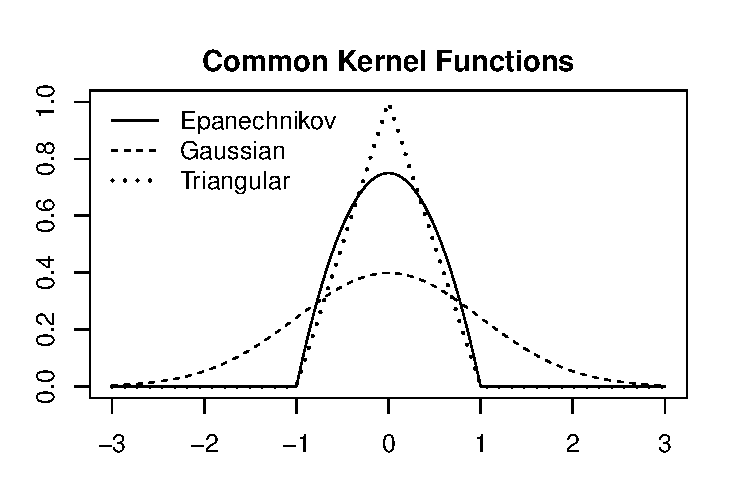
\includegraphics{FinalReport_files/figure-latex/unnamed-chunk-2-1.pdf}
\caption{Three Common Kernel Functions: the solid line is the
Epanechnikov kernel, the dashed line is the standard Gaussian kernel,
and the dotted line is the Triangular kernel}
\end{figure}

The selection of the bandwidth is more important than the selection of a
kernel function. We use the bandwidth to control how much weight we
apply to observations around the \(x\) for which we are evaluating
\(\widehat{f_h}(x)\). If \(h\) is too small, we assign density too
locally, resulting in wiggly estimates; however, if we select \(h\) to
be too large, we spread density too diffusely, smoothing out interesting
features of the data (Givens and Hoeting 2013). We have illustrated the
effect of bandwidth in Figure 2, where we have evaluated
\(\widehat{f_h}(x)\) for 200 points from the \(N(2, 3)\) density.

\begin{figure}[htbp]
\centering
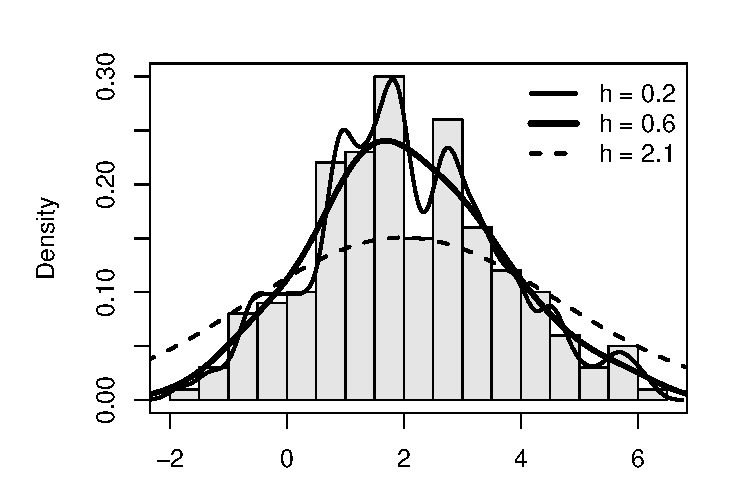
\includegraphics{FinalReport_files/figure-latex/unnamed-chunk-3-1.pdf}
\caption{Kernel density estimates using 3 bandwidths for 500 points from
N(2, 3)}
\end{figure}

We have provided three density estimates in Figure 2, each using a
Gaussian kernel, but different bandwidths. The lighter solid line is too
small of a bandwidth (\(h\) = 0.2), it is too sensitive to local
perturbations. The dashed line is too large of a bandwidth (\(h\) = 2),
so it over-smooths the interesting components of the distribution. The
heavy line (\(h\) = 0.6) seems to be a fairly respectable bandwidth, it
does not over-smooth the data, but it also highlights some of the
interesting features of the data.

\newpage

\section{Methods for evaluating KDE}\label{methods-for-evaluating-kde}

To calculate \(\widehat{f_h}(x)\), we need to compute an estimate for
every observation \(x_i\), based on the \(n-1\) remaining observations
in the data. This computation requires \(n * (n-1)\) computations to
calculate \(\widehat{f_h}(x)\). To get around such a computationally
intensive calculation, possible techniques such as linear binning and
Fast Fourier Transforms are used (both are used in \texttt{R}'s
\texttt{density} function).

\subsection{Evaluating the Fit of $\widehat{f}_h(x)$}

Along with the computation of \(\widehat{f_h}(x)\), it is also important
to assess the quality of \(\hat{f}\) as an estimator of \(f\). One
choice would the be the Integrated Squared Error (ISE):

\[ISE(h) = \int_{-\infty}^{\infty} \left(\hat{f}(x) - f(x)\right)^2dx.\]
ISE calculates the squared error for \emph{this} sample. It might be
reasonable to average ISE over \emph{all} samples, resulting in Mean
Integrated Squared Error (MISE): \(MISE(h) = E\left(ISE(h)\right).\)

We can rewrite \(MISE(h)\) as:

\[MISE(h) = \int_{-\infty}^{\infty}MSE_h\left(\hat{f}(x)\right)dx,\] and
decompose \(MSE\) as \(MSE = bias^2 + var\):

\[MISE(h) = \int_{-\infty}^{\infty} var\left(\widehat{f_h}(x)\right) + bias\left(\widehat{f_h}(x)\right)^2 dx.\]
Givens and Hoeting (2013, 327) say of the distinction between \(ISE\)
and \(MISE\)\footnote{The reader may be interested in our focus on
  squared error, instead of opting for the \(L_1\) norm. While the
  \(L_1\) norm is theoretically appealing, due to its invariance under
  one-to-one smooth transformations, it can be somewhat difficult to
  analyze mathematically. For this reason it is neglected here.}:

\begin{quote}
The distinction is essentially one between the statistical concepts of
loss and risk. Using ISE(h) is conceptually appealing because it
assesses the estimator's performance with the observed data. However,
focusing on MISE(h) is an effective way to approximate ISE-based
evaluation while reflecting the sensible goal of seeking optimal
perfomance on average over many data sets.
\end{quote}

Givens and Hoeting (2013, 331) derived \(E[\widehat{f_h}(x)]\) as:

\[E[\widehat{f_h}(x)] = f(x) + \frac{1}{2} \sigma_K^2f^{''}(x) + o(h^2),\]

where \(\sigma_K^2\) is the variance of \(K\) (\(\int z^2 K(z) dz\)). So
that
\(\left(bias(\widehat{f_h}(x))\right)^2 = \frac{1}{4}\sigma_K^4 (f^{''})^2 + o(h^4)\),
and integrating \(bias^2\) results in:

\[\int bias\left(\hat{f}(x)\right)^2 dx = \frac{1}{4} h^4 \sigma_K^4 R(f^{''}) + o(h^4),\]

where \(R\) is a measure of the roughness of a function g:

\[R(g) = \int_{-\infty}^{\infty}g^2(z) dz.\] Table 1 contains
information about \(\sigma_K^2\) and \(R(K)\) for the Gaussian,
Epanechnikov, and Triangular kernels.

\begin{table}[ht]
\caption{Kernel Function Properties} % title of Table
\centering % used for centering table
\begin{tabular}{l l l l} % centered columns (4 columns)
\hline\hline %inserts double horizontal lines
Name & Function & $R(K)$ & $\sigma_K^2$ \\ [0.5ex] % inserts table
%heading
\hline % inserts single horizontal line
Gaussian & $ K(z) = \phi(z)$ & $\frac{1}{2\sqrt{\pi}}$ & 1 \\ [1.5ex] % inserting body of the table
Epanechnikov & $K(z) = \frac{3}{4}  (1 - z^2)*1(|z| <1)$ & $\frac{3}{5}$ & $\frac{1}{5}$ \\ [1.5ex]
Triangular & $K(z)= (1 - |z|) * 1(|z| < 1)$ & $\frac{2}{3}$ & $\frac{1}{6}$ \\ [1ex] % [1ex] adds vertical space
\hline %inserts single line
\end{tabular}
\label{table:kernprop} % is used to refer this table in the text
\end{table}

It can also be shown that
\(var\left(\hat{f}(x)\right) = \frac{1}{nh}f(x)R(K) + o(\frac{1}{nh})\),
and integrating \(var\) results in:

\[\int var\left(\hat{f}(x)\right)dx = \frac{R(K)}{nh} + o(\frac{1}{nh}).\]

Adding \(bias^2\) and \(var\) together results in:

\[
\begin{aligned}
MISE(h) &= \frac{R(K)}{nh} + o\left(\frac{1}{nh}\right) + \frac{1}{4}h^4 \sigma_K^4R(f^{''}) + o\left(h^4\right) \\
&= AMISE(h) + o\left(\frac{1}{nh} + h^4\right),
\end{aligned}
\] where \(AMISE\) is the Asymptotic Mean Integrated Squared Error. If
\(nh \rightarrow \infty\) and \(h \rightarrow 0\) as
\(n \rightarrow \infty\), then \(MISE(h) \rightarrow 0\).

Inspection of the \(bias^2\) and \(var\) components of \(MISE(h)\) with
respect to the bandwidth \(h\) provides an example of the oft-mentioned
bias-variance tradeoff. Selecting a small value of \(h\) increases
variance by producing a wiggly estimate, but reduces bias, while
selecting a large value of \(h\) reduces the variance of the estimator,
but increases the bias due to over-smoothing. To find an optimal value,
we must balance the bias and variance components of \(MISE\), a typical
theme in statistical inference.

Finding an optimal bandwidth \(h_{AMISE}\), is straightforward using
calculus (ignoring \(o\left(\frac{1}{nh} + h^4\right)\)):

\[
\begin{aligned}
AMISE &= \frac{R(K)}{nh} + \frac{h^4\sigma_K^4R(f^{''})}{4}\\
\frac{dAMISE}{dh} &= \frac{-R(K)}{nh^2} + h^3\sigma_K^4 R(f^{''})\\
0 &= \frac{-R(K)}{n} + h^5 \sigma_K^4 R(f^{''}) \\
h^5 &= \frac{R(K)}{n\sigma_K^4 R(f^{''})} \\
h_{AMISE} &= \left(\frac{R(K)}{n\sigma_K^4R(f^{''})}\right)^{\frac{1}{5}}.
\end{aligned}
\]

All of the components of \(h_{AMISE}\) are known to us, except for
\(R(f^{''})\). The possible choices for bandwidth depend on replacing
\(R(f^{''})\) with some estimate, \(\widehat{R(f^{''})}\). Of
\(R(f^{''})\), Sheather (2004, 589) states:

\begin{quote}
Thus, the functional \(R(f^{''})\) is a measure of the underlying
roughness or curvature. In particular, the larger the value of
\(R(f^{''})\) is, the larger is the value of AMISE (i.e., the more
difficult it is to estimate \(f\)) and the smaller is the value of
\(h_{AMISE}\) (i.e., the smaller the bandwidth needed to capture the
curvature in \(f\)).
\end{quote}

\section{Bandwidth Selection}\label{bandwidth-selection}

\subsection{Unbiased Cross Validation}\label{unbiased-cross-validation}

We can represent integrated squared error as:

\[
ISE(h) = \int \left(\hat{f}_h - f\right) = \int\hat{f}_h^2 - 2\int \hat{f}_hf + \int f^2.
\]

In \(ISE(h)\), only the first two terms rely on \(h\), and the first
term is entirely known. We can estimate the second term
(\(2\int \hat{f}_hf = 2 E(\hat{f}_h)\)) using
\(2/n \sum_{i=1}^{n}\hat{f}_{-i}(x_i)\). Where

\[
\hat{f}_{-i}(x_i) = \frac{1}{h(n-1)}\sum_{j \neq i} K\left(\frac{x_i - x_j}{h}\right)
\]

is the leave-one-out kernel density estimator using all of the data
except \(x_i\).

We then attempt to minimize

\[
UCV(h) = R(\hat{f}) - \frac{2}{n} \sum_{i = 1}^{n} \hat{f}_{-i}(x_i),
\] with respect to \(h\).

\(UCV(h)\) is called the ``unbiased cross-validation'' criterion because
\(E\left[UCV(h) + R(f)\right] = MISE(h)\) (Givens and Hoeting 2013,
333). To estimate the unbiased cross validation bandwidth for a data
vector \texttt{x} in \texttt{R}, a user can write \texttt{bw.ucv(x)}.
Along with ``unbiased cross-validation'', it is sometimes referred to as
``least-squares cross validation'' as it minimizes the integrated
squared error. When we refer to the bandwidth selection, we denote the
bandwidth as \(h_{LSCV}\).

For this report, we have focused on the Gaussian kernel. \(UCV(h)\) has
a straightforward expression (equation 10.23, Givens and Hoeting (2013,
333)) when a Gaussian kernel is used, which makes the computation of
\(h_{LSCV}\) rather tidy.

The unbiasedness of the objective function is a nice feature, but it
comes at the cost of imbuing \(h_{LSCV}\) with excessive variance
(Jones, Marron, and Sheather 1992, 6). This excessive variation is
displayed in the examples section of this report.

\subsection{Silverman's Rule of Thumb}\label{silvermans-rule-of-thumb}

A simpler method relies on selecting an appropriate density to
approximate \(R(f^{''})\) in

\[
h_{AMISE} = \left(\frac{R(K)}{n\sigma_K^4R(f^{''})}\right)^{\frac{1}{5}}.
\]

If we choose \(f\) to be the normal density with mean 0 and variance
\(\sigma^2\), and use a Gaussian kernel, we can express \(h_{AMISE}\)
as:

\[
\begin{aligned}
h_{AMISE} &= \left(\frac{(2\sqrt{\pi})^{-1}}{\frac{3}{8}\pi^{-\frac{1}{2}}\sigma^{-5}}\right)^{1/5} n^{-1/5} \\
&= 1.06\sigma n^{-\frac{1}{5}}.
\end{aligned}
\]

A natural estimate of \(\sigma\) is \(\hat{\sigma}\), the sample
standard deviation. If the true \(f\) deviates from the features of a
normal distribution (for instance, it is multimodal), this approximation
may do a poor job (i.e.~it will oversmooth). A possiblity is to use the
interquartile range, which is a more robust measure of spread. We then
replace \(\hat{sigma}\) with
\(\tilde{\sigma} = min\left[\hat{\sigma}, \frac{IQR(x)}{1.34}\right]\).
This leads to Silverman's rule of thumb:

\[
h_{SROT_1} = 1.06 \tilde{\sigma} n ^ {-\frac{1}{5}}.
\]

In our report, we replace 1.06 in the previous equation with 0.9, so
that \(h_{SROT} = \frac{0.9}{1.06} h_{SROT_1}\). This replacement
dampens some of the oversmoothing that takes place when this method is
used, and attempts to avoid missing bimodality in the distribution
(Silverman 1986, 48). In \texttt{R}, a user can obtain \(h_{SROT_1}\)
for a data vector \texttt{x} by using \texttt{bw.nrd(x)}, and can obtain
\(h_{SROT}\) by using \texttt{bw.nrd0(x)}.

The computation of \(h_{SROT}\) is fairly simple, and requires no
optimzation or cross-validation scheme. The simplicity comes at a cost;
however, since this bandwidth tends to oversmooth the estimate, even
after the IQR correction is made.

\subsection{Sheather-Jones Bandwidth}\label{sheather-jones-bandwidth}

Silverman's rule of thumb relies on selecting a candidate density to
estimate \(R(f^{''})\). Sheather and Jones (1991) opt for a different
approach: empirically estimate \(R(f^{''})\). An empirical estimate of
\(f^{''}\) is formulated as:

\[
\begin{aligned}
\hat{f}''(x) &= \frac{d^2}{dx^2} \left\{\frac{1}{nh_0} \sum_{i=1}^{n} L\left(\frac{x - x_i}{h_0}  \right) \right\}\\
&= \frac{1}{nh_0^3} \sum_{i=1}^{n} L''\left(\frac{x-x_i}{h_0} \right).
\end{aligned}
\]

Where \(h_0\) is another bandiwdth, different from \(h_{opt}\) (and
typically \(h_0 > h_{opt}\) Givens and Hoeting (2013, 336)), and \(L\)
is a kernel function.

To compute the optimal bandwidth \(h_{SJ}\), Sheather and Jones use a
two-step process. First, a simple rule of thumb is used to calculate
\(h_0\). Then \(h_0\) is used to estimate \(R(f^{''})\), which is the
only unknown quantity in the expression for \(h_{AMISE}\). After
plugging in the estimator for \(R(f^{''})\) in the expression for
\(h_{AMISE}\), we arrive at the Sheather-Jones bandwidth. An expression
for the optimal bandwidth when \(L = \phi\) is in the Appendix. This
expression requires an root-finding scheme such as Newton's method.

In simulation studies (summarized in Jones, Marron, and Sheather
(1996)), it was seen that \(h_{SJ}\) tended to be superior to both
\(h_{LSCV}\) and \(h_{SROT}\). In general, \(h_{SJ}\) demonstrates less
variation than \(h_{LSCV}\) and is centered near \(h_{AMISE}\) for easy
to estimate densities. For more difficult densities, \(h_{SJ}\) will
overshoot \(h_{AMISE}\), but is still much smaller than \(h_{SROT}\).
\(h_{SJ}\), then, seems to be a suitable compromise between the
low-variance high-bias \(h_{SROT}\) and the high-variance low-bias
\(h_{LSCV}\).

\subsection{Terrell's Maximal Smoothing
Principle}\label{terrells-maximal-smoothing-principle}

Terrell (1990) opted for a different approach in determining an optimal
bandwidth. Rather than focusing on finding a good estimator of \(f\) or
\(R(f'')\) in the expression for \(h_{AMISE}\), Terrell chose to
determine some function \(g\) that would minimize
\(R(g'') = \int (g '' (x))^2 dx\). By minimizing \(\int (g'')^2\), we
could determine an upper bound for \(h_{opt}\), by using \(g\) as our
estimate for \(f\). Terrell (1990, 472) justifies using the maximally
smoothed bandwidth, because it avoids the tendency of the undersmoothed
density estimate to ``display features such as asymmetries and multiple
modes that could have come about by chance''.

Terrell's estimate is built on the result that the
\(beta(k + 2, k + 2)\) family minimizes \(\int (f^{(k)})^2\) for a given
standard deviation (Terrell 1990, 471). For a kernel with variance 1
(e.g.~the Gaussian kernel), the maximal smoothing bandiwdth is:

\[
h_{MS} =  3 \hat \sigma \left(\frac{R(K)}{35 n} \right)^{\frac{1}{5}}.
\]

The maximal smoothing principle has an intuitive justification, and its
ideas permeate through wider areas of statistical inference, where an
inferential scheme should prevent an analyst from claiming features of a
data set exist that may have arisen by pure chance alone (Terrell 1990,
472).

In terms of kernel density estimation; however, the maximal smoothing
principle provides only an upper bound on the optimal bandwidth.
Silverman's rule of thumb is an over-smoother, and Terrell's maximal
smoothing bandwidth smooths out even more features of the data (Jones,
Marron, and Sheather 1992, 9) than \(h_{SROT}\) does.

\section{\texorpdfstring{Examples Using the \texttt{kde}
Function}{Examples Using the kde Function}}\label{examples-using-the-kde-function}

To examine the four different bandwidth selections we have investigated,
we use four different data vectors to investigate the changes in density
estimation as the data deviates from the normal distribution. Our main
interest is on if the bandwidth options lead to undersmoothing or
oversmoothing of the data.

We plot histograms and density estimates for each of the data vectors
using the \texttt{kde} function (source code available in appendix). The
\texttt{kde} function takes in a data vector, and calculates
\(h_{SROT}\), \(h_{SJ}\), \(h_{LSCV}\), and \(h_{MS}\). It then
calculates \(\widehat{f}_h(x)\). For small data vectors
(\(n \leq 1,000\)), \texttt{kde} will calculate the densities ``by
hand'', using a grid of size 512. For larger data vectors, the function
will use the \texttt{density} function in base \texttt{R}. In addition
to creating plots, the \texttt{kde} function will print the four
bandwidths, and can also return \(\widehat{f}_h(x)\) for an evenly
spaced grid of length 512 for each \(h\).

In each example, we choose a data vector and display the output from
\texttt{kde}. We then attempt to interpret the results, taking special
care to analyze the effect of each bandwidth choice on \(\hat{f}_h\).
Inspecting a kernel density estimate is not an objective task, one
analyst will perceive different features than another. It is important
to present multiple density estimates, and iterate through different
bandwidths to arrive at a more common conclusion.

\subsection{Example 1: 300 samples from $N(2, 2^2)$}

\begin{verbatim}
## Silverman's ROT           LS CV           SJ BW            T MS 
##           0.519           0.648           0.598           0.691
\end{verbatim}

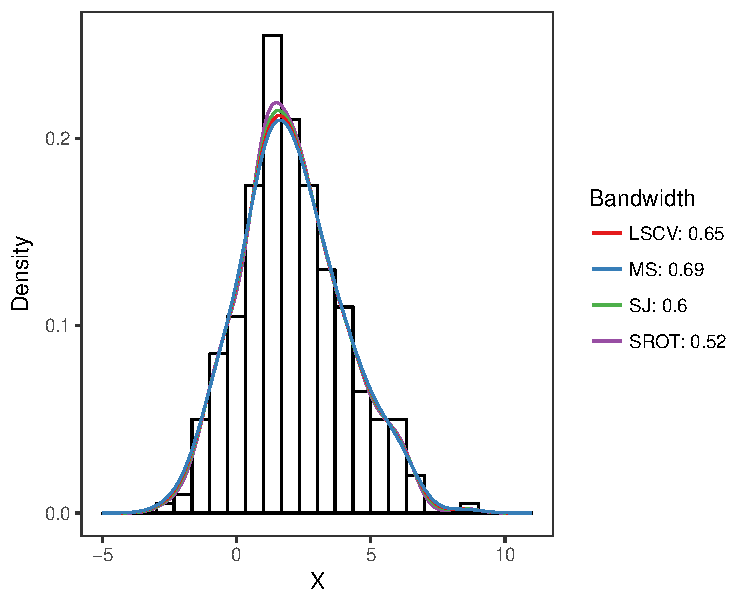
\includegraphics{FinalReport_files/figure-latex/unnamed-chunk-5-1.pdf}

We begin by examining \(\widehat{f}_h(x)\) for a data vector sampled
solely from \(N(2, 2^2)\). In this case, we see that each bandwidth
selection does a fairly good job of estimating the density. \(h_{SROT}\)
relies on a normal approximation, so we would expect this bandwidth to
perform well on this vector. In fact, it is the most aggressive
bandwidth estimator, resulting in the smallest \(h\) value of the four.
A \emph{best bandwidth} is not apparent from these results.

\subsection{Example 2: 50/50 Mixture of $N(0, 1)$ and $N(4, 2^2)$}

\begin{verbatim}
## Silverman's ROT           LS CV           SJ BW            T MS 
##           0.742           0.562           0.515           0.944
\end{verbatim}

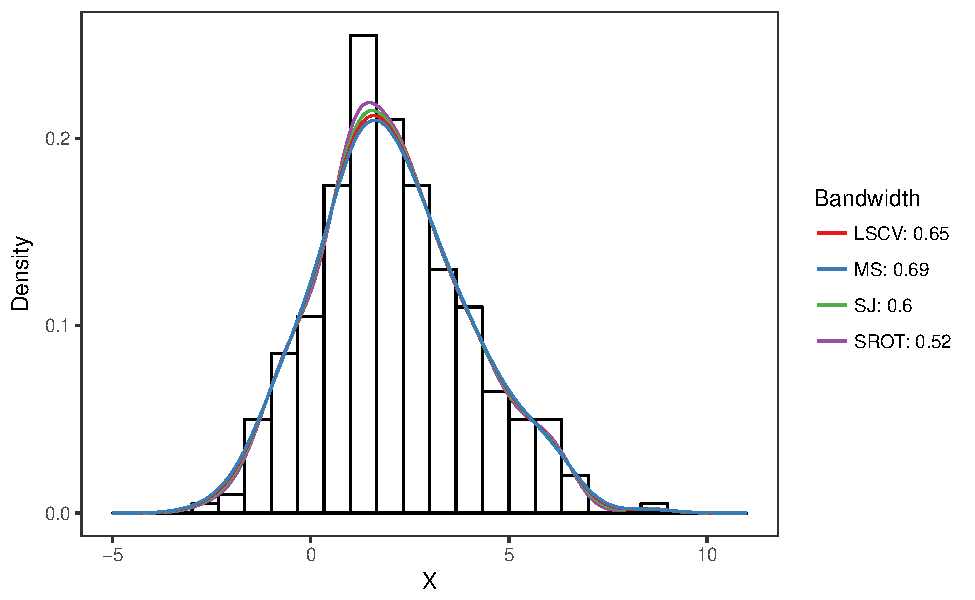
\includegraphics{FinalReport_files/figure-latex/unnamed-chunk-6-1.pdf}

Moving on to a somewhat harder density to estimate, we simulate a 50/50
distribution coming from \(N(0,1)\) and \(N(2, 2^2)\). \(h_{SJ}\) and
\(h_{LSCV}\) both seem to capture the bimodality of the distribution
quite well. \(h_{SROT}\) smooths out some of the interesting features,
but the bimodality is still somewhat detectable. \(h_{MS}\) oversmooths
disastrously - without knowing the underlying structure of the data, it
would not be obvious that the data came from a bimodal distribution.

\subsection{Example 3: Mixture of $\Gamma(\alpha = 1, \beta = 1/20)$, $\Gamma(\alpha = 4, \beta = 1/5)$, $\Gamma(\alpha = 20, \beta = 1)$}

A mixture of gamma distributions may seem like a ``toy'' example, but
the gamma distribution can be very helpful in modeling rainfall (e.g.
Husak, Michaelsen, and Funk (2007)).

\begin{verbatim}
## Silverman's ROT           LS CV           SJ BW            T MS 
##           2.374           1.382           2.241           4.514
\end{verbatim}

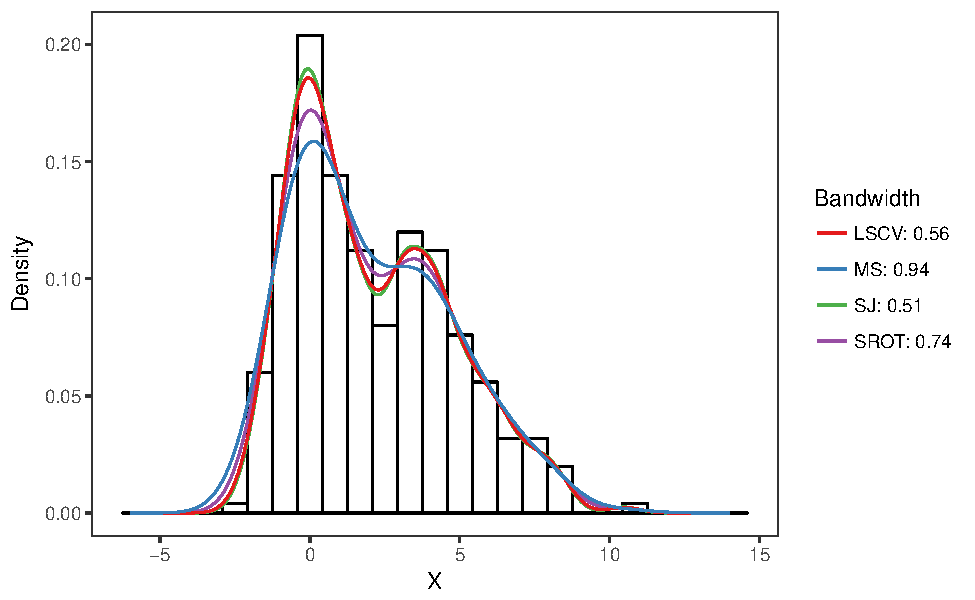
\includegraphics{FinalReport_files/figure-latex/unnamed-chunk-7-1.pdf}

Here we see the excessive variation caused by using \(h_{LSCV}\). The
density estimate provided by \(h_{LSCV}\) is far too wiggly to be useful
for a data analyst. We also see that \(h_{MS}\) provides a much smoother
estimate than the those proposed by Silverman and Sheather and Jones, it
seems that it is too conservative. The best bandwidth would take a value
somewhere in the range between \(h_{SJ}\) and \(h_{MS}\).

\subsection{Example 4: Old Faithful Waiting Time}

\begin{verbatim}
## Silverman's ROT           LS CV           SJ BW            T MS 
##           3.998           2.190           2.560           5.081
\end{verbatim}

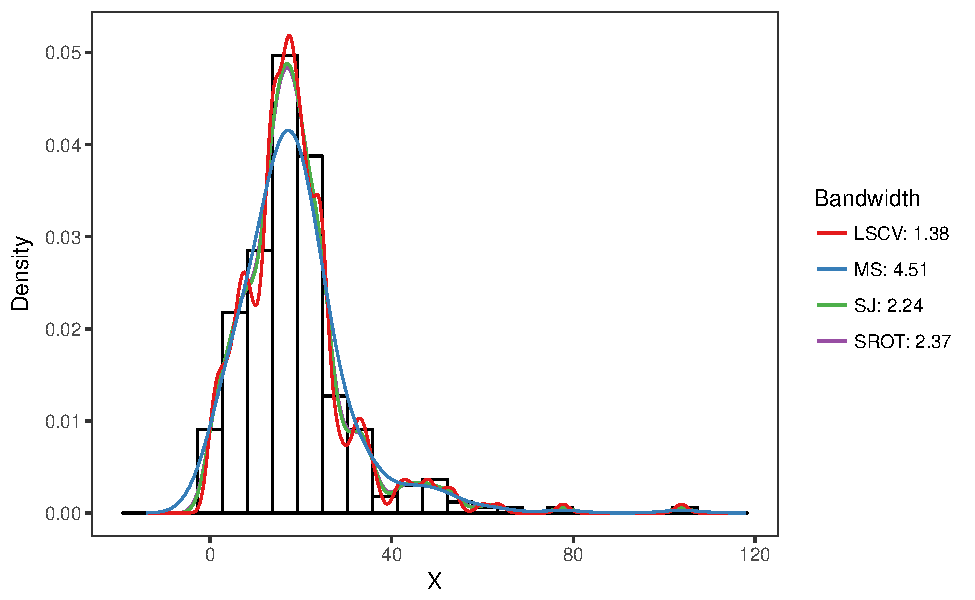
\includegraphics{FinalReport_files/figure-latex/unnamed-chunk-8-1.pdf}

Using data from Azzalini and Bowman (1990), contained in the
\textbf{\texttt{MASS}} package, we calculate the kernel density estimate
for the waiting time for eruptions from August 1 to August 15, 1985 at
the Old Faithful geyser in Yellowstone National Park, Wyoming.

Each bandwidth choice seems to capture the bimodality in the
distribution of waiting times with varying levels of success.
\(h_{LSCV}\) may be too aggressive, while \(h_{MS}\) does not reach far
enough up the left-side peak. \(h_{SJ}\) and \(h_{LSCV}\) seem grouped
together and \(h_{SROT}\) and \(h_{MS}\) seem grouped together as well.
Between \(h_{SJ}\) and \(h_{LSCV}\), we would want to choose the more
conservative bandwidth, which is \(h_{SJ}\). Conversely, between
\(h_{MS}\) and \(h_{SROT}\), we would want to choose the more aggressive
bandwidth, which is \(h_{SROT}\).

\section{Conclusion}\label{conclusion}

\section{Question}\label{question}

Using the \texttt{density} function and the beer data
(\texttt{abv.complete}, which are the alcohol by volume measures for the
top 250 beers as rated by BeerAdvocate.com) provided below, estimate a
95\% pointwise bootstrapped percentile interval. Additionally, use the
approximate variance function \(\tilde{V}\) given by Jann (2007, 2) to
estimate a 95\% pointwise confidence interval. Create plots using
\texttt{bw.SJ} and \texttt{bw.nrd0}.

\[\tilde{V}\left(\widehat{f_K}(x;h)\right) = \frac{1}{nh}R(K) \widehat{f_K}(x;h) - \frac{1}{n} \widehat{f_K}(x;h)^2\]

\begin{Shaded}
\begin{Highlighting}[]
\CommentTok{# data comes from the ABV of beer advocate's top 250 beers for 2016}
\CommentTok{# 2 beers have missing abv data}
\CommentTok{# quick R script to read in the .csv}
\KeywordTok{library}\NormalTok{(RCurl)}
\NormalTok{git_file <-}\StringTok{ }
\KeywordTok{getURL}\NormalTok{(}\StringTok{"https://raw.githubusercontent.com/bgstieber/Top250Beer/master/Top250Beers.csv"}\NormalTok{)}
\NormalTok{beer_data <-}\StringTok{ }\KeywordTok{read.csv}\NormalTok{(}\DataTypeTok{text =} \NormalTok{git_file, }\DataTypeTok{stringsAsFactors =} \OtherTok{FALSE}\NormalTok{)}
\NormalTok{abv.complete <-}\StringTok{ }\NormalTok{beer_data[!}\KeywordTok{is.na}\NormalTok{(beer_data$ABV), ]$ABV}
\end{Highlighting}
\end{Shaded}

\section{Solution}\label{solution}

\subsection{Bootstrap percentile
interval}\label{bootstrap-percentile-interval}

\begin{Shaded}
\begin{Highlighting}[]
\CommentTok{#function that computes the 95% pointwise percentile interval}
\NormalTok{boot_dens <-}\StringTok{ }\NormalTok{function(x, from, to, B, bw)\{}
    
    
    \NormalTok{orig_dens <-}\StringTok{ }\KeywordTok{density}\NormalTok{(x, }\DataTypeTok{from =} \NormalTok{from, }\DataTypeTok{to =} \NormalTok{to, }\DataTypeTok{bw =} \NormalTok{bw)}
    
    \NormalTok{boot_dens <-}\StringTok{ }\KeywordTok{matrix}\NormalTok{(}\DecValTok{0}\NormalTok{, }\DataTypeTok{ncol =} \NormalTok{B, }\DataTypeTok{nrow =} \KeywordTok{length}\NormalTok{(orig_dens$x))}

    \NormalTok{for(i in }\DecValTok{1}\NormalTok{:B)\{}
        \NormalTok{boot.x <-}\StringTok{ }\KeywordTok{sample}\NormalTok{(x, }\KeywordTok{length}\NormalTok{(x), }\DataTypeTok{replace =} \NormalTok{T)}
        \NormalTok{boot.density <-}\StringTok{ }\KeywordTok{density}\NormalTok{(boot.x, }\DataTypeTok{from =} \NormalTok{from, }\DataTypeTok{to =} \NormalTok{to, }\DataTypeTok{bw =} \NormalTok{bw)}
        \NormalTok{boot_dens[,i] <-}\StringTok{ }\NormalTok{boot.density$y}
    \NormalTok{\}}
    
    \NormalTok{lower <-}\StringTok{ }\KeywordTok{apply}\NormalTok{(boot_dens, }\DecValTok{1}\NormalTok{, function(mat) }\KeywordTok{quantile}\NormalTok{(mat, .}\DecValTok{025}\NormalTok{))}
    \NormalTok{upper <-}\StringTok{ }\KeywordTok{apply}\NormalTok{(boot_dens, }\DecValTok{1}\NormalTok{, function(mat) }\KeywordTok{quantile}\NormalTok{(mat, .}\DecValTok{975}\NormalTok{))}
    
    \KeywordTok{data.frame}\NormalTok{(}\DataTypeTok{grid =} \NormalTok{orig_dens$x,}
               \DataTypeTok{yhat =} \NormalTok{orig_dens$y,}
               \DataTypeTok{lower =} \NormalTok{lower,}
               \DataTypeTok{upper =} \NormalTok{upper)}
    
\NormalTok{\}}
\end{Highlighting}
\end{Shaded}

\begin{Shaded}
\begin{Highlighting}[]
\NormalTok{range_abv <-}\StringTok{ }\KeywordTok{range}\NormalTok{(abv.complete)}
\NormalTok{range_abv <-}\StringTok{ }\NormalTok{range_abv +}\StringTok{ }\KeywordTok{c}\NormalTok{(-.}\DecValTok{5}\NormalTok{, .}\DecValTok{5}\NormalTok{) }\CommentTok{#wiggle room}
    
\KeywordTok{set.seed}\NormalTok{(}\DecValTok{1984}\NormalTok{)}

\NormalTok{boot.abv.SJ <-}\StringTok{ }\KeywordTok{boot_dens}\NormalTok{(}\DataTypeTok{x =} \NormalTok{abv.complete, }\DataTypeTok{from =} \NormalTok{range_abv[}\DecValTok{1}\NormalTok{],}
                      \DataTypeTok{to =} \NormalTok{range_abv[}\DecValTok{2}\NormalTok{], }\DataTypeTok{B =} \DecValTok{1500}\NormalTok{, }\DataTypeTok{bw =} \StringTok{'SJ'}\NormalTok{)}

\NormalTok{boot.abv.nrd0 <-}\StringTok{ }\KeywordTok{boot_dens}\NormalTok{(}\DataTypeTok{x =} \NormalTok{abv.complete, }\DataTypeTok{from =} \NormalTok{range_abv[}\DecValTok{1}\NormalTok{],}
                      \DataTypeTok{to =} \NormalTok{range_abv[}\DecValTok{2}\NormalTok{], }\DataTypeTok{B =} \DecValTok{1500}\NormalTok{, }\DataTypeTok{bw =} \StringTok{'nrd0'}\NormalTok{)}

\KeywordTok{ggplot}\NormalTok{(boot.abv.SJ, }\KeywordTok{aes}\NormalTok{(}\DataTypeTok{x =} \NormalTok{grid))+}
\StringTok{    }\KeywordTok{geom_ribbon}\NormalTok{(}\KeywordTok{aes}\NormalTok{(}\DataTypeTok{ymin =} \NormalTok{lower, }\DataTypeTok{ymax =} \NormalTok{upper),}
                \DataTypeTok{alpha =} \NormalTok{.}\DecValTok{2}\NormalTok{)+}
\StringTok{    }\KeywordTok{geom_line}\NormalTok{(}\KeywordTok{aes}\NormalTok{(}\DataTypeTok{y =} \NormalTok{yhat),}
              \DataTypeTok{colour =} \StringTok{'#b70101'}\NormalTok{)+}
\StringTok{    }\KeywordTok{geom_rug}\NormalTok{(}\DataTypeTok{data =} \KeywordTok{data.frame}\NormalTok{(abv.complete), }
             \KeywordTok{aes}\NormalTok{(}\DataTypeTok{x =} \NormalTok{abv.complete, }\DataTypeTok{y =} \FloatTok{0.001}\NormalTok{),}
             \DataTypeTok{inherit.aes =} \OtherTok{FALSE}\NormalTok{, }\DataTypeTok{sides =} \StringTok{'b'}\NormalTok{)+}
\StringTok{    }\KeywordTok{xlab}\NormalTok{(}\StringTok{'ABV'}\NormalTok{)+}\KeywordTok{ylab}\NormalTok{(}\StringTok{'Density'}\NormalTok{)+}
\StringTok{    }\KeywordTok{ggtitle}\NormalTok{(}\StringTok{'ABV Density and 95% Boostrapped Percentile Interval'}\NormalTok{,}
            \DataTypeTok{subtitle =} \StringTok{'Sheather - Jones Bandwidth'}\NormalTok{)}
\end{Highlighting}
\end{Shaded}

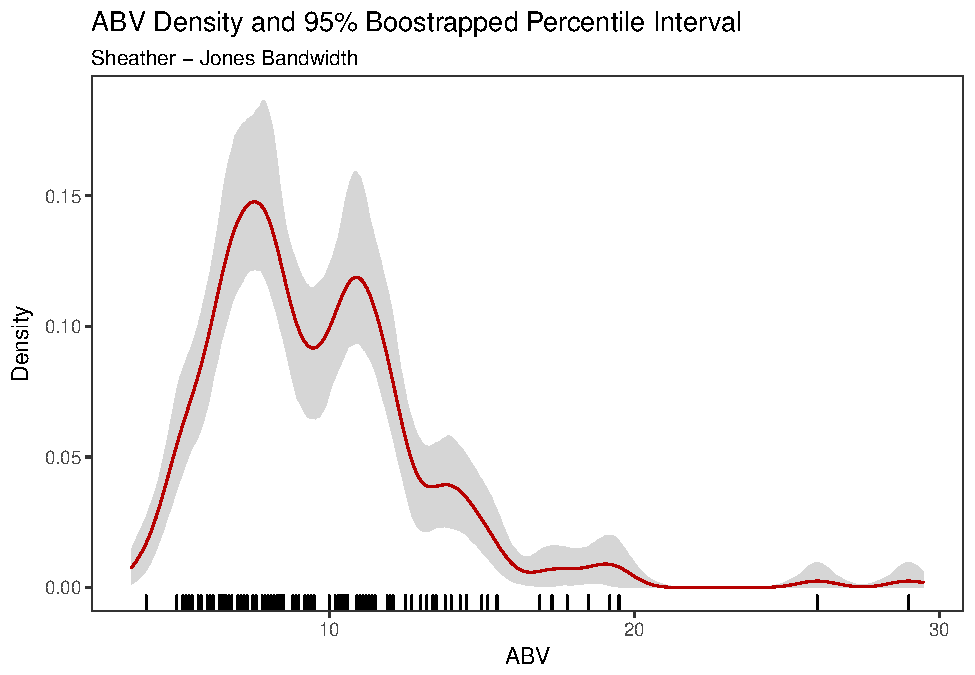
\includegraphics{FinalReport_files/figure-latex/unnamed-chunk-12-1.pdf}

\begin{Shaded}
\begin{Highlighting}[]
\KeywordTok{ggplot}\NormalTok{(boot.abv.nrd0, }\KeywordTok{aes}\NormalTok{(}\DataTypeTok{x =} \NormalTok{grid))+}
\StringTok{    }\KeywordTok{geom_ribbon}\NormalTok{(}\KeywordTok{aes}\NormalTok{(}\DataTypeTok{ymin =} \NormalTok{lower, }\DataTypeTok{ymax =} \NormalTok{upper),}
                \DataTypeTok{alpha =} \NormalTok{.}\DecValTok{2}\NormalTok{)+}
\StringTok{    }\KeywordTok{geom_line}\NormalTok{(}\KeywordTok{aes}\NormalTok{(}\DataTypeTok{y =} \NormalTok{yhat),}
              \DataTypeTok{colour =} \StringTok{'#b70101'}\NormalTok{)+}
\StringTok{    }\KeywordTok{geom_rug}\NormalTok{(}\DataTypeTok{data =} \KeywordTok{data.frame}\NormalTok{(abv.complete), }
             \KeywordTok{aes}\NormalTok{(}\DataTypeTok{x =} \NormalTok{abv.complete, }\DataTypeTok{y =} \FloatTok{0.001}\NormalTok{),}
             \DataTypeTok{inherit.aes =} \OtherTok{FALSE}\NormalTok{, }\DataTypeTok{sides =} \StringTok{'b'}\NormalTok{)+}
\StringTok{    }\KeywordTok{xlab}\NormalTok{(}\StringTok{'ABV'}\NormalTok{)+}\KeywordTok{ylab}\NormalTok{(}\StringTok{'Density'}\NormalTok{)+}
\StringTok{    }\KeywordTok{ggtitle}\NormalTok{(}\StringTok{'ABV Density and 95% Boostrapped Percentile Interval'}\NormalTok{,}
            \DataTypeTok{subtitle =} \StringTok{"Silverman's ROT Bandwidth"}\NormalTok{)}
\end{Highlighting}
\end{Shaded}

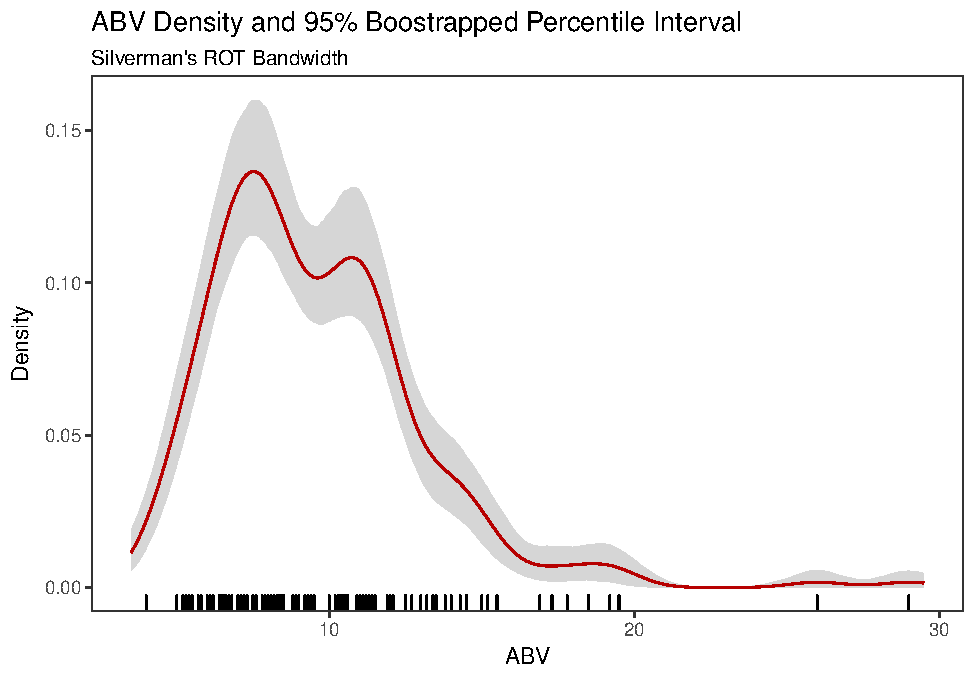
\includegraphics{FinalReport_files/figure-latex/unnamed-chunk-12-2.pdf}

\subsection{Approximate Confidence
Interval}\label{approximate-confidence-interval}

\begin{Shaded}
\begin{Highlighting}[]
\NormalTok{app_var <-}\StringTok{ }\NormalTok{function(x, bw)\{}
    \NormalTok{R <-}\StringTok{ }\DecValTok{1} \NormalTok{/}\StringTok{ }\NormalTok{(}\DecValTok{2} \NormalTok{*}\StringTok{ }\KeywordTok{sqrt}\NormalTok{(pi)) }\CommentTok{# assume gaussian}
    \NormalTok{h <-}\StringTok{ }\KeywordTok{ifelse}\NormalTok{(bw ==}\StringTok{ 'SJ'}\NormalTok{, }\KeywordTok{bw.SJ}\NormalTok{(x), }\KeywordTok{bw.nrd0}\NormalTok{(x))}
    \NormalTok{n <-}\StringTok{ }\KeywordTok{length}\NormalTok{(x)}
    \NormalTok{range_x <-}\StringTok{ }\KeywordTok{range}\NormalTok{(x)}
    \NormalTok{range_x <-}\StringTok{ }\NormalTok{range_x *}\StringTok{ }\FloatTok{1.01} \CommentTok{#wiggle room}
    \NormalTok{dens_x <-}\StringTok{ }\KeywordTok{density}\NormalTok{(x, }\DataTypeTok{from =} \NormalTok{range_x[}\DecValTok{1}\NormalTok{], }\DataTypeTok{to =} \NormalTok{range_x[}\DecValTok{2}\NormalTok{],}
                      \DataTypeTok{kernel =} \StringTok{'gaussian'}\NormalTok{, }\DataTypeTok{bw =} \NormalTok{h)}
    
    \NormalTok{var.dens <-}\StringTok{ }\NormalTok{(}\DecValTok{1} \NormalTok{/}\StringTok{ }\NormalTok{(n *}\StringTok{ }\NormalTok{h)) *}\StringTok{ }\NormalTok{R *}\StringTok{ }\NormalTok{dens_x$y -}\StringTok{ }\NormalTok{((}\DecValTok{1} \NormalTok{/}\StringTok{ }\NormalTok{n) *}\StringTok{ }\NormalTok{(dens_x$y) ^}\StringTok{ }\DecValTok{2}\NormalTok{)}
    
    \NormalTok{lower <-}\StringTok{ }\NormalTok{dens_x$y -}\StringTok{ }\NormalTok{(}\DecValTok{2} \NormalTok{*}\StringTok{ }\KeywordTok{sqrt}\NormalTok{(var.dens))}
    \NormalTok{upper <-}\StringTok{ }\NormalTok{dens_x$y +}\StringTok{ }\NormalTok{(}\DecValTok{2} \NormalTok{*}\StringTok{ }\KeywordTok{sqrt}\NormalTok{(var.dens))}
    
    \KeywordTok{data.frame}\NormalTok{(}\DataTypeTok{grid =} \NormalTok{dens_x$x,}
               \DataTypeTok{yhat =} \NormalTok{dens_x$y,}
               \DataTypeTok{lower =} \NormalTok{lower,}
               \DataTypeTok{upper =} \NormalTok{upper)}
\NormalTok{\}}
\end{Highlighting}
\end{Shaded}

\begin{Shaded}
\begin{Highlighting}[]
\NormalTok{app.abv.SJ <-}\StringTok{ }\KeywordTok{app_var}\NormalTok{(}\DataTypeTok{x =} \NormalTok{abv.complete, }\DataTypeTok{bw =} \StringTok{'SJ'}\NormalTok{)}
\NormalTok{app.abv.nrd0 <-}\StringTok{ }\KeywordTok{app_var}\NormalTok{(}\DataTypeTok{x =} \NormalTok{abv.complete, }\DataTypeTok{bw =} \StringTok{'nrd0'}\NormalTok{)}

\KeywordTok{ggplot}\NormalTok{(app.abv.SJ, }\KeywordTok{aes}\NormalTok{(}\DataTypeTok{x =} \NormalTok{grid))+}
\StringTok{    }\KeywordTok{geom_ribbon}\NormalTok{(}\KeywordTok{aes}\NormalTok{(}\DataTypeTok{ymin =} \NormalTok{lower, }\DataTypeTok{ymax =} \NormalTok{upper),}
                \DataTypeTok{alpha =} \NormalTok{.}\DecValTok{2}\NormalTok{)+}
\StringTok{    }\KeywordTok{geom_line}\NormalTok{(}\KeywordTok{aes}\NormalTok{(}\DataTypeTok{y =} \NormalTok{yhat), }\DataTypeTok{colour =} \StringTok{'#b70101'}\NormalTok{)+}
\StringTok{        }\KeywordTok{geom_rug}\NormalTok{(}\DataTypeTok{data =} \KeywordTok{data.frame}\NormalTok{(abv.complete), }
             \KeywordTok{aes}\NormalTok{(}\DataTypeTok{x =} \NormalTok{abv.complete, }\DataTypeTok{y =} \FloatTok{0.001}\NormalTok{),}
             \DataTypeTok{inherit.aes =} \OtherTok{FALSE}\NormalTok{, }\DataTypeTok{sides =} \StringTok{'b'}\NormalTok{)+}
\StringTok{    }\KeywordTok{xlab}\NormalTok{(}\StringTok{'ABV'}\NormalTok{)+}
\StringTok{    }\KeywordTok{ylab}\NormalTok{(}\StringTok{'Density'}\NormalTok{)+}
\StringTok{    }\KeywordTok{ggtitle}\NormalTok{(}\StringTok{'ABV Density and 95% Pointwise CI'}\NormalTok{,}
            \DataTypeTok{subtitle =} \StringTok{'Sheather - Jones Bandwidth'}\NormalTok{)}
\end{Highlighting}
\end{Shaded}

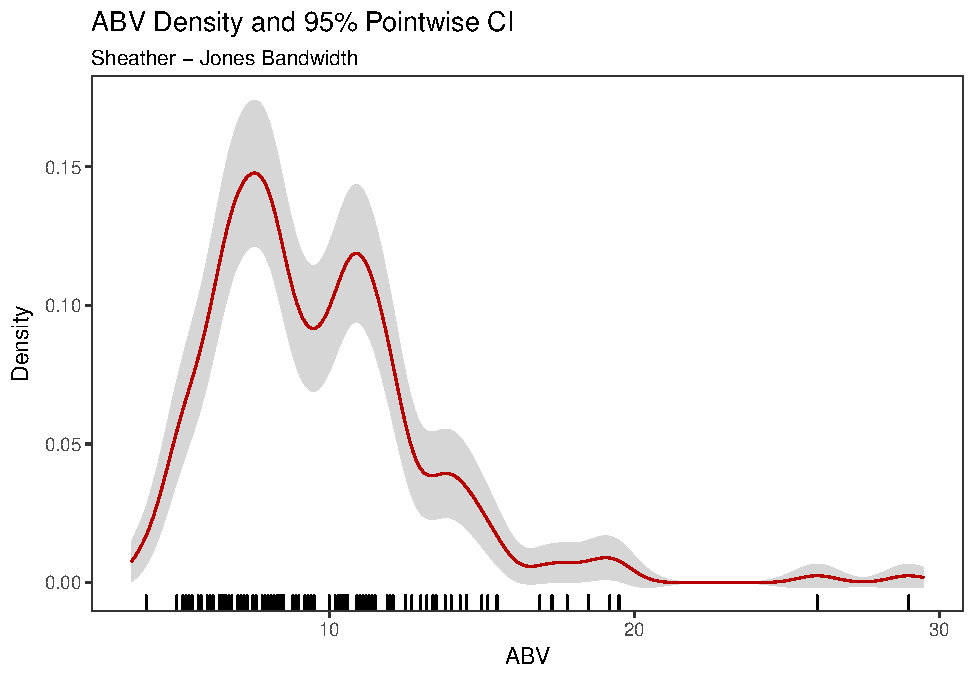
\includegraphics{FinalReport_files/figure-latex/unnamed-chunk-14-1.pdf}

\begin{Shaded}
\begin{Highlighting}[]
\KeywordTok{ggplot}\NormalTok{(app.abv.nrd0, }\KeywordTok{aes}\NormalTok{(}\DataTypeTok{x =} \NormalTok{grid))+}
\StringTok{    }\KeywordTok{geom_ribbon}\NormalTok{(}\KeywordTok{aes}\NormalTok{(}\DataTypeTok{ymin =} \NormalTok{lower, }\DataTypeTok{ymax =} \NormalTok{upper),}
                \DataTypeTok{alpha =} \NormalTok{.}\DecValTok{2}\NormalTok{)+}
\StringTok{    }\KeywordTok{geom_line}\NormalTok{(}\KeywordTok{aes}\NormalTok{(}\DataTypeTok{y =} \NormalTok{yhat), }\DataTypeTok{colour =} \StringTok{'#b70101'}\NormalTok{)+}
\StringTok{        }\KeywordTok{geom_rug}\NormalTok{(}\DataTypeTok{data =} \KeywordTok{data.frame}\NormalTok{(abv.complete), }
             \KeywordTok{aes}\NormalTok{(}\DataTypeTok{x =} \NormalTok{abv.complete, }\DataTypeTok{y =} \FloatTok{0.001}\NormalTok{),}
             \DataTypeTok{inherit.aes =} \OtherTok{FALSE}\NormalTok{, }\DataTypeTok{sides =} \StringTok{'b'}\NormalTok{)+}
\StringTok{    }\KeywordTok{xlab}\NormalTok{(}\StringTok{'ABV'}\NormalTok{)+}
\StringTok{    }\KeywordTok{ylab}\NormalTok{(}\StringTok{'Density'}\NormalTok{)+}
\StringTok{    }\KeywordTok{ggtitle}\NormalTok{(}\StringTok{'ABV Density and 95% Pointwise CI'}\NormalTok{,}
            \DataTypeTok{subtitle =} \StringTok{"Silverman's ROT Bandwidth"}\NormalTok{)}
\end{Highlighting}
\end{Shaded}

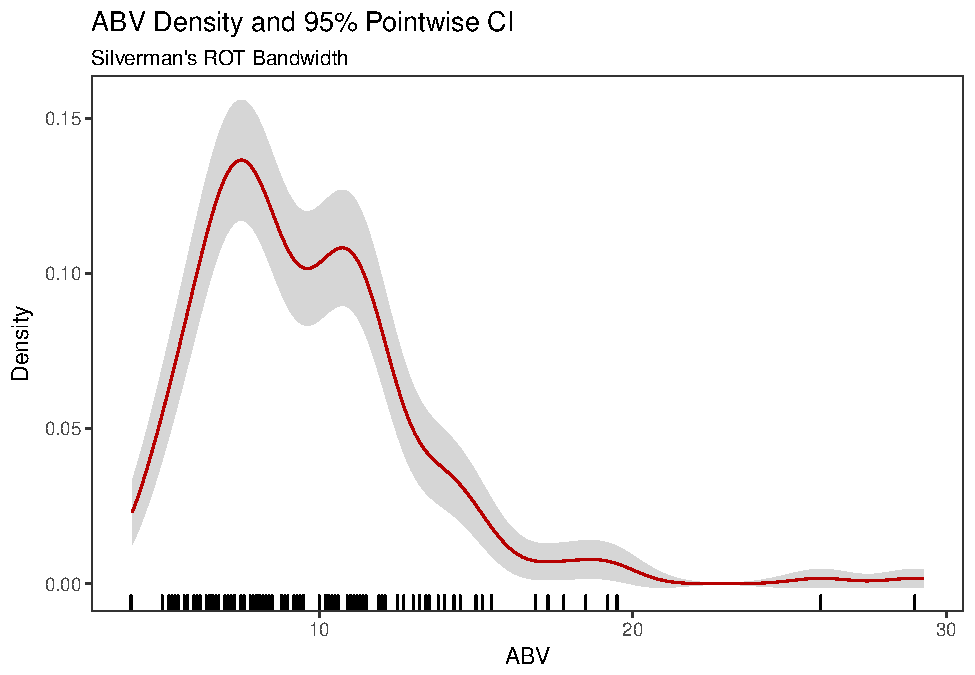
\includegraphics{FinalReport_files/figure-latex/unnamed-chunk-14-2.pdf}

\section{Appendix}\label{appendix}

\subsection{\texorpdfstring{\texttt{kde} function in
\texttt{R}}{kde function in R}}\label{kde-function-in-r}

\begin{Shaded}
\begin{Highlighting}[]
\NormalTok{Knorm <-}\StringTok{ }\NormalTok{function(u) }\KeywordTok{dnorm}\NormalTok{(u)}
\NormalTok{kde <-}\StringTok{ }\NormalTok{function (x, }\DataTypeTok{grid =} \DecValTok{512}\NormalTok{, }\DataTypeTok{give_dens =} \OtherTok{FALSE}\NormalTok{) }
\NormalTok{\{}
    \KeywordTok{require}\NormalTok{(dplyr)}
    \KeywordTok{require}\NormalTok{(ggplot2)}
    
    \NormalTok{n <-}\StringTok{ }\KeywordTok{length}\NormalTok{(x)}
    
    \NormalTok{h.SROT =}\StringTok{ }\FloatTok{0.9} \NormalTok{*}\StringTok{ }\KeywordTok{min}\NormalTok{(}\KeywordTok{c}\NormalTok{(}\KeywordTok{IQR}\NormalTok{(x) /}\StringTok{ }\FloatTok{1.34}\NormalTok{, }\KeywordTok{sd}\NormalTok{(x))) *}\StringTok{ }\NormalTok{(n)^(-}\DecValTok{1}\NormalTok{/}\DecValTok{5}\NormalTok{)}
    \NormalTok{h.LSCV =}\StringTok{ }\KeywordTok{bw.ucv}\NormalTok{(x, }\DataTypeTok{lower =} \NormalTok{.}\DecValTok{05} \NormalTok{*}\StringTok{ }\NormalTok{h.SROT, }\DataTypeTok{upper =} \FloatTok{1.2} \NormalTok{*}\StringTok{ }\NormalTok{h.SROT)}
    \NormalTok{h.SJ =}\StringTok{ }\KeywordTok{bw.SJ}\NormalTok{(x)}
    \NormalTok{h.MS =}\StringTok{ }\DecValTok{3} \NormalTok{*}\StringTok{ }\NormalTok{((}\DecValTok{2} \NormalTok{*}\StringTok{ }\KeywordTok{sqrt}\NormalTok{(pi))^(-}\DecValTok{1}\NormalTok{) /}\StringTok{ }\NormalTok{(}\DecValTok{35} \NormalTok{*}\StringTok{ }\NormalTok{n))^(}\DecValTok{1}\NormalTok{/}\DecValTok{5}\NormalTok{) *}\StringTok{ }\KeywordTok{sd}\NormalTok{(x)}
    \NormalTok{h_vec <-}\StringTok{ }\KeywordTok{c}\NormalTok{(h.SROT, h.LSCV, h.SJ, h.MS)}
    
    \NormalTok{max_h <-}\StringTok{ }\KeywordTok{max}\NormalTok{(h_vec)}
    \NormalTok{low_grid <-}\StringTok{ }\KeywordTok{floor}\NormalTok{(}\KeywordTok{min}\NormalTok{(x) -}\StringTok{ }\NormalTok{max_h *}\StringTok{ }\DecValTok{3}\NormalTok{)}
    \NormalTok{high_grid <-}\StringTok{ }\KeywordTok{ceiling}\NormalTok{(}\KeywordTok{max}\NormalTok{(x) +}\StringTok{ }\NormalTok{max_h *}\StringTok{ }\DecValTok{3}\NormalTok{)}
    
    
    \KeywordTok{print}\NormalTok{(}\KeywordTok{c}\NormalTok{(}\StringTok{"Silverman's ROT"} \NormalTok{=}\StringTok{ }\KeywordTok{round}\NormalTok{(h.SROT, }\DecValTok{3}\NormalTok{), }
            \StringTok{'LS CV'} \NormalTok{=}\StringTok{ }\KeywordTok{round}\NormalTok{(h.LSCV, }\DecValTok{3}\NormalTok{),}
            \StringTok{'SJ BW'} \NormalTok{=}\StringTok{ }\KeywordTok{round}\NormalTok{(h.SJ, }\DecValTok{3}\NormalTok{),}
            \StringTok{'T MS'} \NormalTok{=}\StringTok{ }\KeywordTok{round}\NormalTok{(h.MS, }\DecValTok{3}\NormalTok{)))}
    
    
    \NormalTok{if(n >}\StringTok{ }\DecValTok{1000}\NormalTok{)\{}
        \KeywordTok{message}\NormalTok{(}\KeywordTok{paste0}\NormalTok{(}\StringTok{'Note: x too large (n = '}\NormalTok{, n, }
                       \StringTok{' > 1000). Using `density` instead'}\NormalTok{))}
        
        \NormalTok{all_dens <-}\StringTok{ }\KeywordTok{do.call}\NormalTok{(}\StringTok{'cbind'}\NormalTok{, }
                            \KeywordTok{lapply}\NormalTok{(h_vec, function(bw)}
                                \KeywordTok{density}\NormalTok{(}\DataTypeTok{x =} \NormalTok{x, }\DataTypeTok{from =} \NormalTok{low_grid, }\DataTypeTok{to =} \NormalTok{high_grid,}
                                        \DataTypeTok{bw=} \NormalTok{bw)$y))}
        
        
        \NormalTok{dens_SNR <-}\StringTok{ }\KeywordTok{density}\NormalTok{(x, }\DataTypeTok{bw =} \NormalTok{h.SNR,}
                            \DataTypeTok{from =} \NormalTok{low_grid,}
                            \DataTypeTok{to =} \NormalTok{high_grid)}
        
        \NormalTok{sum_results <-}\StringTok{ }\KeywordTok{data.frame}\NormalTok{(}
            \DataTypeTok{X_grid =} \NormalTok{dens_SNR$x,}
            \DataTypeTok{kde_hSROT =} \NormalTok{all_dens[,}\DecValTok{1}\NormalTok{],}
            \DataTypeTok{kde_hSJ =} \NormalTok{all_dens[,}\DecValTok{3}\NormalTok{],}
            \DataTypeTok{kde_hLSCV =} \NormalTok{all_dens[,}\DecValTok{2}\NormalTok{],}
            \DataTypeTok{kde_hMS =} \NormalTok{all_dens[,}\DecValTok{4}\NormalTok{]}
        \NormalTok{)}
        
    \NormalTok{\}else\{}
        
        \NormalTok{grid_vals <-}\StringTok{ }\KeywordTok{seq}\NormalTok{(low_grid, high_grid, }\DataTypeTok{length.out =} \NormalTok{grid)}
        
        \NormalTok{grid_df <-}\StringTok{ }\KeywordTok{expand.grid}\NormalTok{(}\DataTypeTok{x =} \NormalTok{x, }\DataTypeTok{grid =} \NormalTok{grid_vals)}
        
        
        
        \NormalTok{newx.hsrot <-}\StringTok{ }\NormalTok{(grid_df[,}\DecValTok{2}\NormalTok{] -}\StringTok{ }\NormalTok{grid_df[,}\DecValTok{1}\NormalTok{]) /}\StringTok{ }\NormalTok{h.SROT}
        \NormalTok{newx.hsj <-}\StringTok{ }\NormalTok{(grid_df[,}\DecValTok{2}\NormalTok{] -}\StringTok{ }\NormalTok{grid_df[,}\DecValTok{1}\NormalTok{]) /}\StringTok{ }\NormalTok{h.SJ}
        \NormalTok{newx.hLSCV <-}\StringTok{ }\NormalTok{(grid_df[,}\DecValTok{2}\NormalTok{] -}\StringTok{ }\NormalTok{grid_df[,}\DecValTok{1}\NormalTok{]) /}\StringTok{ }\NormalTok{h.LSCV}
        \NormalTok{newx.hMS <-}\StringTok{ }\NormalTok{(grid_df[,}\DecValTok{2}\NormalTok{] -}\StringTok{ }\NormalTok{grid_df[,}\DecValTok{1}\NormalTok{]) /}\StringTok{ }\NormalTok{h.MS}
        
        \NormalTok{grid_df[,}\DecValTok{3}\NormalTok{] <-}\StringTok{ }\NormalTok{(}\DecValTok{1} \NormalTok{/}\StringTok{ }\NormalTok{(n *}\StringTok{ }\NormalTok{h.SROT)) *}\StringTok{ }\KeywordTok{Knorm}\NormalTok{(newx.hsrot)}
        \NormalTok{grid_df[,}\DecValTok{4}\NormalTok{] <-}\StringTok{ }\NormalTok{(}\DecValTok{1} \NormalTok{/}\StringTok{ }\NormalTok{(n *}\StringTok{ }\NormalTok{h.SJ)) *}\StringTok{ }\KeywordTok{Knorm}\NormalTok{(newx.hsj)}
        \NormalTok{grid_df[,}\DecValTok{5}\NormalTok{] <-}\StringTok{ }\NormalTok{(}\DecValTok{1} \NormalTok{/}\StringTok{ }\NormalTok{(n *}\StringTok{ }\NormalTok{h.LSCV)) *}\StringTok{ }\KeywordTok{Knorm}\NormalTok{(newx.hLSCV)}
        \NormalTok{grid_df[,}\DecValTok{6}\NormalTok{] <-}\StringTok{ }\NormalTok{(}\DecValTok{1} \NormalTok{/}\StringTok{ }\NormalTok{(n *}\StringTok{ }\NormalTok{h.MS)) *}\StringTok{ }\KeywordTok{Knorm}\NormalTok{(newx.hMS)}
        
        
        \KeywordTok{names}\NormalTok{(grid_df) <-}\StringTok{ }\KeywordTok{c}\NormalTok{(}
            \StringTok{"X_act"}\NormalTok{, }
            \StringTok{"X_grid"}\NormalTok{, }
            \StringTok{'kde_hSROT'}\NormalTok{,}
            \StringTok{'kde_hSJ'}\NormalTok{,}
            \StringTok{'kde_hLSCV'}\NormalTok{,}
            \StringTok{'kde_hMS'}
        \NormalTok{)}
        
        
        \NormalTok{sum_results <-}\StringTok{ }
\StringTok{            }\NormalTok{grid_df %>%}
\StringTok{            }\KeywordTok{group_by}\NormalTok{(X_grid) %>%}
\StringTok{            }\KeywordTok{summarise}\NormalTok{(}\DataTypeTok{kde_hSROT =} \KeywordTok{sum}\NormalTok{(kde_hSROT),}
                      \DataTypeTok{kde_hSJ =} \KeywordTok{sum}\NormalTok{(kde_hSJ),}
                      \DataTypeTok{kde_hLSCV =} \KeywordTok{sum}\NormalTok{(kde_hLSCV),}
                      \DataTypeTok{kde_hMS =} \KeywordTok{sum}\NormalTok{(kde_hMS))}
    \NormalTok{\}}
    
    
    \NormalTok{p1 <-}\StringTok{ }\KeywordTok{ggplot}\NormalTok{()+}
\StringTok{        }\KeywordTok{geom_histogram}\NormalTok{(}\DataTypeTok{data =} \OtherTok{NULL}\NormalTok{, }\KeywordTok{aes}\NormalTok{(}\DataTypeTok{x =} \NormalTok{x, }\DataTypeTok{y =} \NormalTok{..density..),}
                       \DataTypeTok{bins =} \FloatTok{1.4} \NormalTok{*}\StringTok{ }\KeywordTok{ceiling}\NormalTok{(}\KeywordTok{sqrt}\NormalTok{(n)),}
                       \DataTypeTok{fill =} \OtherTok{NA}\NormalTok{, }\DataTypeTok{colour =} \StringTok{'black'}\NormalTok{)+}
\StringTok{        }\KeywordTok{geom_line}\NormalTok{(}\DataTypeTok{data =} \NormalTok{sum_results, }\KeywordTok{aes}\NormalTok{(}\DataTypeTok{x =} \NormalTok{X_grid, }\DataTypeTok{y =} \NormalTok{kde_hSROT,}
                                          \DataTypeTok{colour =} \KeywordTok{paste}\NormalTok{(}\StringTok{'SROT:'}\NormalTok{, }\KeywordTok{round}\NormalTok{(h.SROT, }\DecValTok{2}\NormalTok{))))+}
\StringTok{        }\KeywordTok{geom_line}\NormalTok{(}\DataTypeTok{data =} \NormalTok{sum_results, }\KeywordTok{aes}\NormalTok{(}\DataTypeTok{x =} \NormalTok{X_grid, }\DataTypeTok{y =} \NormalTok{kde_hSJ,}
                                          \DataTypeTok{colour =} \KeywordTok{paste}\NormalTok{(}\StringTok{'SJ:'}\NormalTok{, }\KeywordTok{round}\NormalTok{(h.SJ, }\DecValTok{2}\NormalTok{))))+}
\StringTok{        }\KeywordTok{geom_line}\NormalTok{(}\DataTypeTok{data =} \NormalTok{sum_results, }\KeywordTok{aes}\NormalTok{(}\DataTypeTok{x =} \NormalTok{X_grid, }\DataTypeTok{y =} \NormalTok{kde_hLSCV,}
                                          \DataTypeTok{colour =} \KeywordTok{paste}\NormalTok{(}\StringTok{'LSCV:'}\NormalTok{, }\KeywordTok{round}\NormalTok{(h.LSCV, }\DecValTok{2}\NormalTok{)))) +}
\StringTok{        }\KeywordTok{geom_line}\NormalTok{(}\DataTypeTok{data =} \NormalTok{sum_results, }\KeywordTok{aes}\NormalTok{(}\DataTypeTok{x =} \NormalTok{X_grid, }\DataTypeTok{y =} \NormalTok{kde_hMS,}
                                          \DataTypeTok{colour =} \KeywordTok{paste}\NormalTok{(}\StringTok{'MS:'}\NormalTok{, }\KeywordTok{round}\NormalTok{(h.MS, }\DecValTok{2}\NormalTok{))))+}
\StringTok{        }\KeywordTok{xlab}\NormalTok{(}\StringTok{'X'}\NormalTok{) +}\StringTok{ }\KeywordTok{ylab}\NormalTok{(}\StringTok{'Density'}\NormalTok{)+}
\StringTok{        }\KeywordTok{theme_bw}\NormalTok{()+}
\StringTok{        }\KeywordTok{theme}\NormalTok{(}\DataTypeTok{panel.grid =} \KeywordTok{element_blank}\NormalTok{())+}
\StringTok{        }\KeywordTok{scale_colour_brewer}\NormalTok{(}\DataTypeTok{palette =} \StringTok{'Set1'}\NormalTok{,}
                            \DataTypeTok{name =} \StringTok{'Bandwidth'}\NormalTok{)}
    \KeywordTok{plot}\NormalTok{(p1)}
    
    \NormalTok{if(give_dens)\{}
        \KeywordTok{return}\NormalTok{(sum_results)}
    \NormalTok{\}}
\NormalTok{\}}
\end{Highlighting}
\end{Shaded}

\subsection{Expression for Sheather-Jones
Bandwidth}\label{expression-for-sheather-jones-bandwidth}

As found in Givens and Hoeting (2013, 337), Sheather-Jones bandwidth can
be found by solving the equation (using \(L = \phi\)):

\[
\left( \frac{R(K)}{n\sigma^4_K\hat{R}_{\hat{\alpha}(h)}(f'')} \right)^{1/5} - h = 0,
\]

where:

\[
\begin{aligned}
\hat{R}_{\hat{\alpha}(h)}(f'') &= \frac{1}{n(n-1)\alpha^5}\sum_{i = 1}^{n}\sum_{j=1}^{n}\phi^{(4)}\left(\frac{x_i - x_j}{\alpha}\right), \\
\hat{\alpha}(h) &= \left(\frac{6\sqrt{2}h^5\hat{R}_a(f'')}{\hat{R}_b(f''')}\right)^{1/7},\\
\hat{R}_a(f'') &= \frac{1}{n(n-1)a^5}\sum_{i = 1}^{n}\sum_{j=1}^{n}\phi^{(4)}\left(\frac{x_i - x_j}{a}\right), \\
\hat{R}_b(f'') &= \frac{1}{n(n-1)b^7}\sum_{i = 1}^{n}\sum_{j=1}^{n}\phi^{(6)}\left(\frac{x_i - x_j}{b}\right), \\
a &= \frac{0.920 IQR}{n^{1/7}} \\
b &= \frac{0.912 IQR}{n^{1/9}},
\end{aligned}
\]

where \(IQR\) is the interquartile range of the data, and \(\phi^{(i)}\)
is the ith derivative of the standard normal density function. To
determine the Sheather-Jones bandwidth in \texttt{R}, a user can write
\texttt{bw.SJ(x)}, which uses the \texttt{uniroot} function to perform
the root-finding.

\section*{References}\label{references}
\addcontentsline{toc}{section}{References}

\hypertarget{refs}{}
\hypertarget{ref-Bowman1990}{}
Azzalini, A, and A Bowman. 1990. ``A Look at Some Data on the Old
Faithful Geyer.'' \emph{Journal of the Royal Statistical Society} 39
(3): 357--65.

\hypertarget{ref-Givens2013}{}
Givens, Geof, and Jennifer Hoeting. 2013. \emph{Computational
Statistics}. 2nd ed. John Wiley \& Sons.

\hypertarget{ref-Husak2007}{}
Husak, Gregory J., Joel Michaelsen, and Chris Funk. 2007. ``Use of the
gamma distribution to represent monthly rainfall in Africa for drought
monitoring applications.'' \emph{International Journal of Climatology}
27.7 (June 2007): 935--44.
doi:\href{https://doi.org/10.1002/joc}{10.1002/joc}.

\hypertarget{ref-Jann2007}{}
Jann, Ben. 2007. ``Univariate kernel density estimation.''
\emph{Statistical Software Component}, no. 3.
\url{http://fmwww.bc.edu/RePEc/bocode/k/kdens.pdf}.

\hypertarget{ref-Jones1992}{}
Jones, M. C., J. S. Marron, and Simon J. Sheather. 1992. ``Progress in
data-based bandwidth selection for Kernel density estimation.''
\emph{Computational Statistics} 11 (3): 337--81.

\hypertarget{ref-Jones1996}{}
---------. 1996. ``A Brief Survey of Bandwidth Selection for Density
Estimation.'' \emph{Journal of the American Statistical Association} 91
(433): 401--7.
doi:\href{https://doi.org/10.1080/01621459.1996.10476701}{10.1080/01621459.1996.10476701}.

\hypertarget{ref-Sheather2004}{}
Sheather, Simon J. 2004. ``Density Estimation.'' \emph{Stat. Sci.} 19
(4): 588--97.
doi:\href{https://doi.org/10.1214/088342304000000297}{10.1214/088342304000000297}.

\hypertarget{ref-Sheather1991}{}
Sheather, Simon J., and M. C. Jones. 1991. ``A Reliable Data-Based
Bandwidth Selection Method for Kernel Density Estimation.''
\emph{Journal of the Royal Statistical Society} 53 (3): 683--90.

\hypertarget{ref-Silverman1986}{}
Silverman, Bernard W. 1986. \emph{Density Estimation for Statistics and
Data Analysis}. CRC press.

\hypertarget{ref-Terrell1990}{}
Terrell, George R. 1990. ``The Maximal Smoothing Principle in Density
Estimation.'' \emph{Journal of the American Statistical Association} 85
(410): 470--77.
doi:\href{https://doi.org/10.2307/2289786}{10.2307/2289786}.


\end{document}
